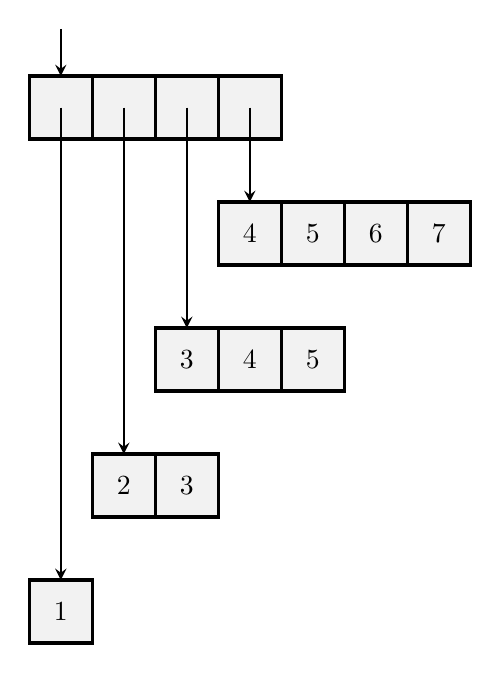
\begin{tikzpicture}[x=8mm, y=-8mm, node distance=0 cm,outer sep = 0pt]
  \tikzstyle{node}=[
    draw,
    rectangle,
    minimum height=8mm,
    minimum width=8mm,
    fill=black!5,
    anchor=center,
    very thick
  ]
  \tikzstyle{arrow} = [thick,->,>=stealth, draw=black]
  
  \node[node] (outer1) at (1,1) {};
  \node[node] (outer2) at (2,1) {};
  \node[node] (outer3) at (3,1) {};
  \node[node] (outer4) at (4,1) {};
  \draw[arrow] (1,-0.25) -- (outer1.north);
  
  \node[node] (inner11) at (4,3) {4};
  \node[node] (inner12) at (5,3) {5};
  \node[node] (inner13) at (6,3) {6};
  \node[node] (inner14) at (7,3) {7};
  \draw[arrow] (outer4.center) -- (inner11.north);
  
  \node[node] (inner21) at (3,5) {3};
  \node[node] (inner22) at (4,5) {4};
  \node[node] (inner23) at (5,5) {5};
  \draw[arrow] (outer3.center) -- (inner21.north);
  
  \node[node] (inner31) at (2,7) {2};
  \node[node] (inner32) at (3,7) {3};
  \draw[arrow] (outer2.center) -- (inner31.north);
  
  \node[node] (inner41) at (1,9) {1};
  \draw[arrow] (outer1.center) -- (inner41.north);
\end{tikzpicture}
